\documentclass[A4]{kulakreport}
\usepackage[dutch]{babel}
\usepackage{xcolor}
\title{Handleiding \textit{automated microplate dispenser}}
\author{Team ELISA\\
Matthias Derez - Maxime Dujardin - Korneel Verkens - Seppe Vilain}
\date{\today}


\begin{document}
	\maketitle
	\tableofcontents
	\newpage
\chapter{voorwoord}
\section{beetje kutten}

Dit is de handleiding voor de \textit{automated microplate dispenser} die door Team ELISA gebouwd werd tijdens het vak 'Probleemoplossen en ontwerpen, deel 3'. In deze handleiding wordt in detail beschreven hoe men de machine moet installeren en gebruiken. Verder worden ook oplossingen uitgelegd voor mogelijke problemen die kunnen opduiken bij het gebruik van de machine.

beetje brielen wie we zijn waarom we deze machine gemaakt hebben en vooral waarom we de handleiding gemaakt hebben aka domme gasten van chemie gaan het anders weer niet kunnen 
LOSERS

\chapter{Installatie}
\section{Hardware}
\label{sectie hardware}
Het apparaat wordt bediend via een computerscherm en -muis. Het computerscherm wordt via een HDMI-kabel verbonden met de microcontroller in de groene box zoals aangegeven op Figuur \ref{fig:HDMI}. De computermuis wordt verbonden via de USB-aansluiting zoals weergegeven in Figuur \ref{fig:USB}. Wanneer het scherm en de muis verbonden zijn met de microcontroller zullen deze automatisch verbinding maken. Het is aan te raden deze aangesloten te laten, om te vermijden dat er bedrading los komt en om slijtage aan het toestel te voorkomen. \\
De zwarte stekker in Figuur \ref{fig:stekker} die uit de groene box komt dient men in een wandcontactdoos te stoppen.
\begin{figure}
	\centering
	\begin{minipage}{.5\textwidth}
		\centering
		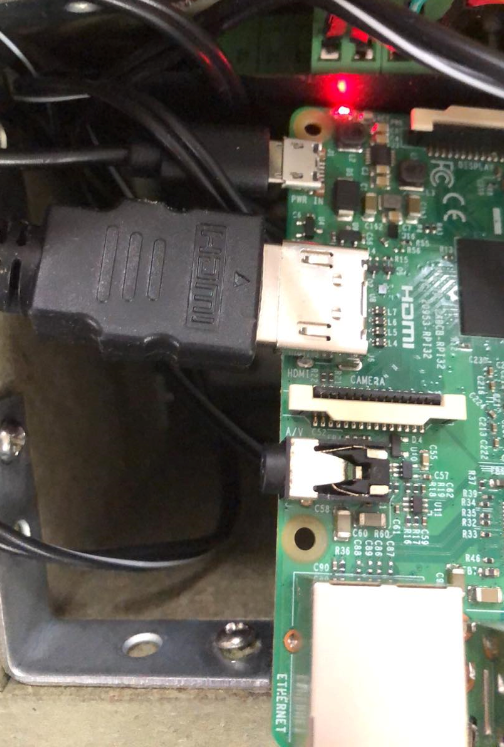
\includegraphics[width=.4\linewidth]{HDMI.png}
		\caption{Aansluiting HDMI-kabel scherm}
		\label{fig:HDMI}
	\end{minipage}%
	\begin{minipage}{.5\textwidth}
		\centering
		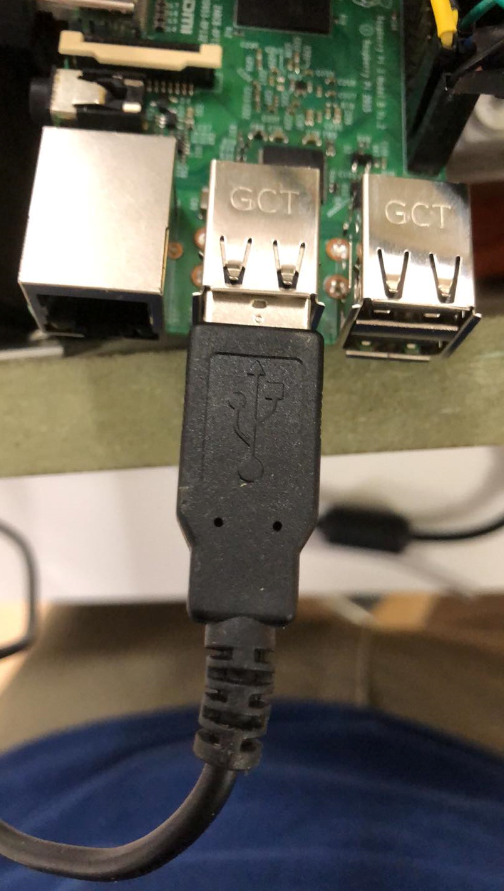
\includegraphics[width=.4\linewidth]{USB.png}
		\caption{Aansluiting USB-kabel muis}
		\label{fig:USB}
	\end{minipage}
\end{figure}
\begin{figure}[h]
	\centering
	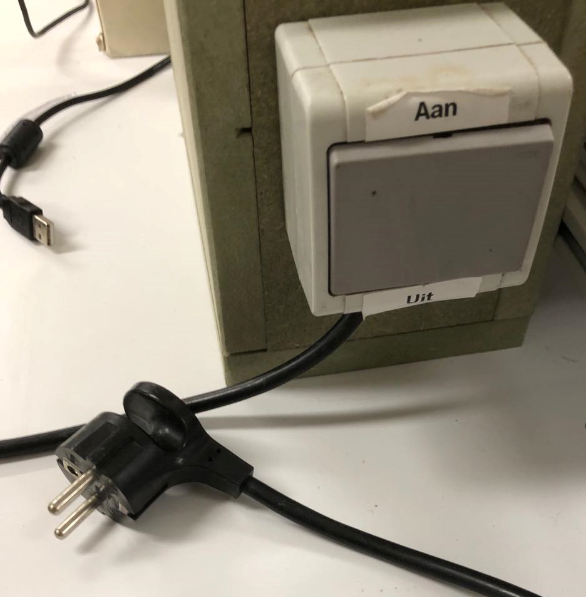
\includegraphics[width=0.5\textwidth]{stekker.png}
	\caption{Zwarte stekker}
	\label{fig:stekker}
	
\end{figure} 



%Om de Automated Microplate Dispenser (verder afgekort als AMD) te kunnen gebruiken, zal men een scherm met hdmi aansluiten en een muis met usb aansluiting nodig hebben. \\
%Deze moet men bevestigen aan de microcontroller, deze bevind zich in de groene box aan 
%de zijkant van de AMD. De hdmi sluit men aan zoals aangeduid op figuur \ref{figuur1} en de muis zoals aangeduid op figuur \ref{figuur2}. \\


%Wanneer deze aangesloten zijn zullen die automatisch verbinden met de microcontroller. Het is aan te raden deze aangesloten te laten, om slijtage te vermijden aan de microcontroller en de AMD zelf. Ook moet men de AMD zelf nog inpluggen in het stopcontact. Uit de groene box loopt een zwarte snoer met een stekker die in het stopcontact moet gestopt worden.\\ \\
%\color{red} hier enkele figuren invoegen dat ze zien wat we bedoelen (ref figuur1 en 2)
%\color{black}
\section{Vloeistof}

Vooraleer men het toestel opstart, dient men de te gebruiken vloeistof klaar te hebben staan. Er kunnen twee verschillende soorten vloeistof gebruikt worden: men kan namelijk de linkse rij \textit{microplates} vullen met een andere vloeistof dan de rechtse rij. Aan de linker- en rechterkant van het apparaat hangen twee zwarte pompen, deze zijn gelabeld als 'pomp links' en 'pomp rechts' (zie FIGUUR). Aan beide pompen hangt een plastic buisje bevestigd wiens uiteinden zich aan de rechterkant van de machine bevinden. Indien men ervoor kiest om één vloeistof te gebruiken, plaatst men de uiteinden van beide buisjes in dezelfde erlenmeyer. Indien met twee vloeistoffen wil gewerkt worden, plaatst men beide uiteinden in twee verschillende erlenmeyers. \\ Wanneer vorige stappen goed uitgevoerd zijn, is het toestel klaar voor gebruik.

\chapter{Opstarten}
\section{Opstarten van het programma}
Om de automatic microplate dispenser op te starten, plaatst men de stekker in hetstopcontact en brengt men de schakelaar aan de groene box in de 'Aan'-positie (zie Figuur \ref{fig:schakelaar}, zorg er zeker voor dat het scherm en de muis verbonden zijn aan de microcontroller zoals beschreven in \ref{sectie hardware}). Vervolgens wacht men enkele ogenblikken tot het startscherm van de automatic microplate dispenser zich op het scherm bevindt. Vooraleer dit zal gebeuren, verschijnt er witte code op het zwarte scherm, dit is volledig normaal. 

\begin{figure}[h]
	\centering
	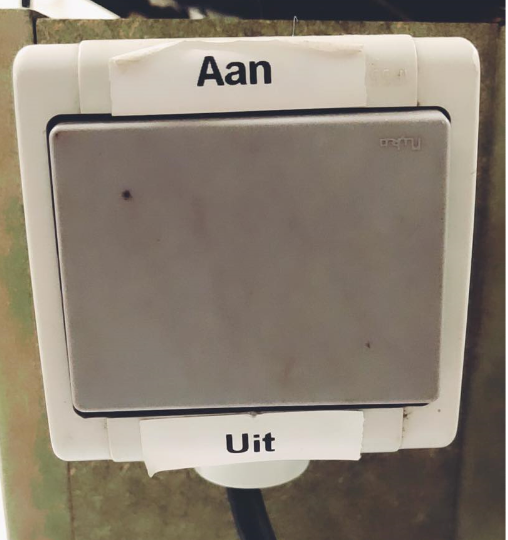
\includegraphics[width=0.5\textwidth]{schakelaar.png}
	\caption{Schakelaar in 'Aan'-positie}
	\label{fig:schakelaar}
	
\end{figure} 



\chapter{Afsluiten}

\chapter{Programma}

\chapter{Mogelijke problemen}
eerst schaaltjes vullen voor de stroom aan te zetten moest er iets mis gaan

\chapter{Onderhoud}

\end{document}